% 12 variables in here:
% u_1 = 0.0, h_1 = 10.0, U_1 = 0.0, H_1 = 10.0, u_2 = 0.0, h_2 = 9.0, U_2 = 0.0, H_2 = 10.0, u_3 = 0.0, h_3 = 10.0, U_3 = 0.0, H_3 = 10.0
\begin{figure}[h!t]
\centering

  \subfigure[Height of point $p_1^L$] {
    \label{subfig:height-p1-three-points-p2-height-decreased}
    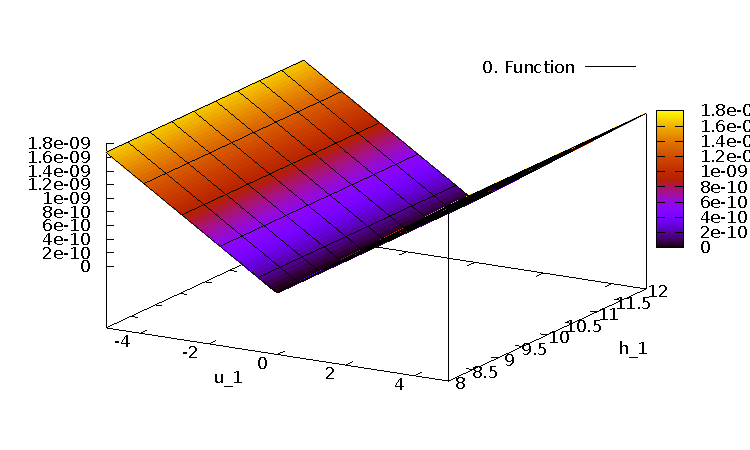
\includegraphics[scale=\zoomfactor]{{{3_punkte_2_hoehe_verringert/x_y_0.0_10.0_0.0_9.0_0.0_10.0_0.0_10.0_0.0_10.0f0}}}  
    %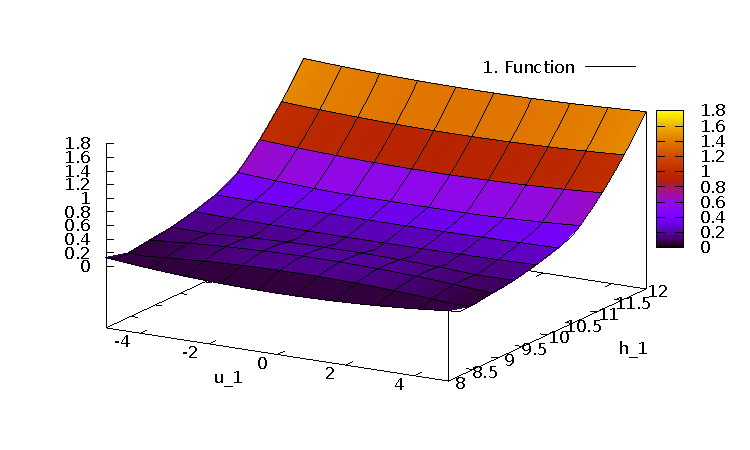
\includegraphics[scale=\zoomfactor]{{{3_punkte_2_hoehe_verringert/x_y_0.0_10.0_0.0_9.0_0.0_10.0_0.0_10.0_0.0_10.0f1}}}  
  }
  \subfigure[Impulse of point $p_1^L$] {
    %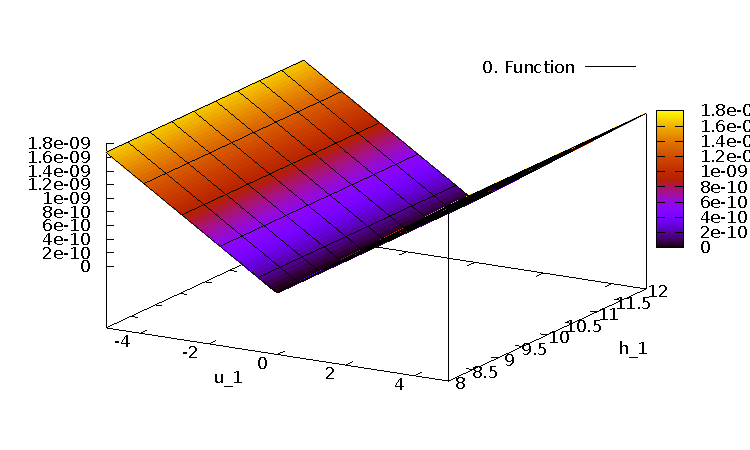
\includegraphics[scale=\zoomfactor]{{{3_punkte_2_hoehe_verringert/x_y_0.0_10.0_0.0_9.0_0.0_10.0_0.0_10.0_0.0_10.0f0}}}  
    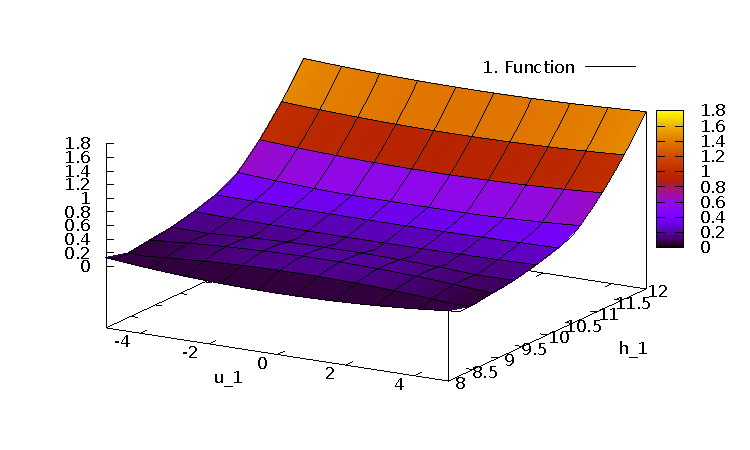
\includegraphics[scale=\zoomfactor]{{{3_punkte_2_hoehe_verringert/x_y_0.0_10.0_0.0_9.0_0.0_10.0_0.0_10.0_0.0_10.0f1}}}  
  }

  % \subfigure[Impulse of point $p_2^L$] {
  %   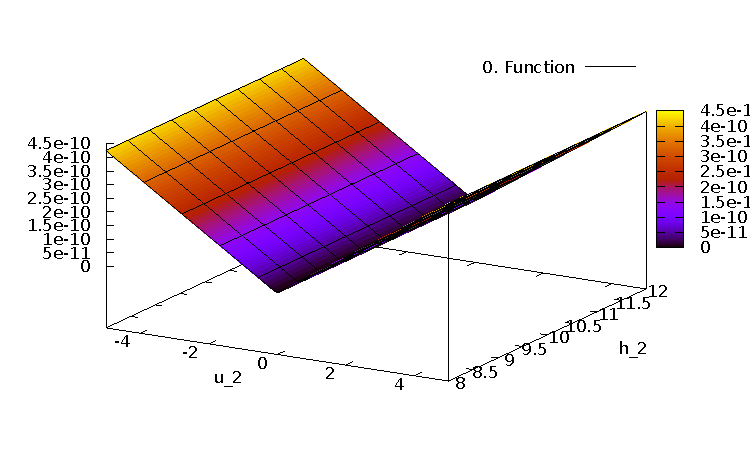
\includegraphics[scale=\zoomfactor]{{{3_punkte_2_hoehe_verringert/0.0_10.0_0.0_10.0_x_y_0.0_10.0_0.0_10.0_0.0_10.0f0}}}  
  %   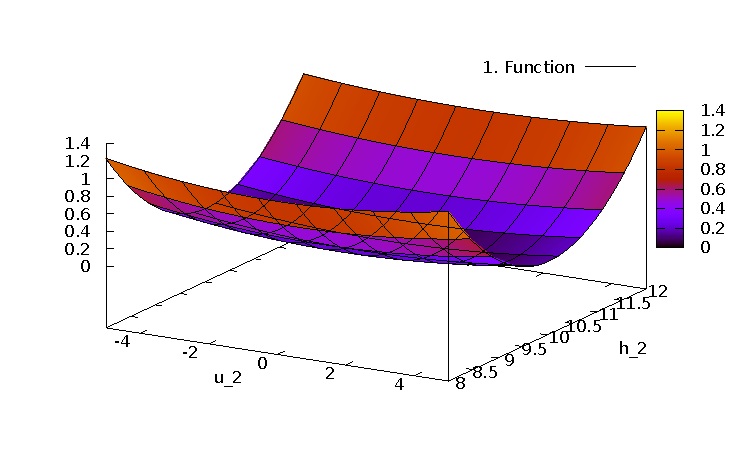
\includegraphics[scale=\zoomfactor]{{{3_punkte_2_hoehe_verringert/0.0_10.0_0.0_10.0_x_y_0.0_10.0_0.0_10.0_0.0_10.0f1}}}  
  % }

  \subfigure[Impulse of point $p_3^L$] {
    %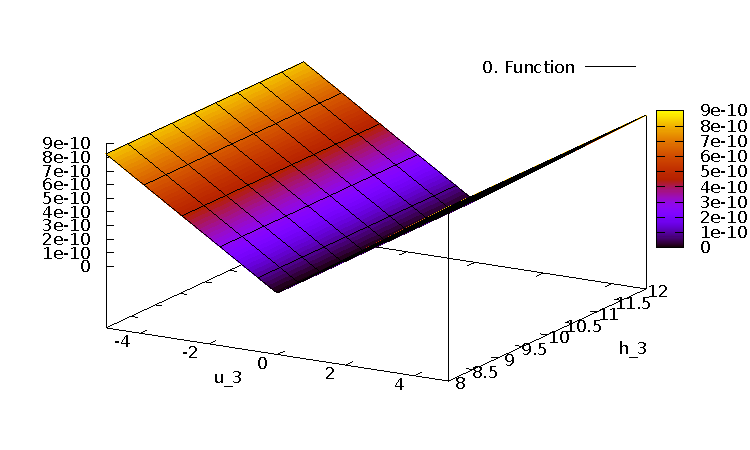
\includegraphics[scale=\zoomfactor]{{{3_punkte_2_hoehe_verringert/0.0_10.0_0.0_10.0_0.0_9.0_0.0_10.0_x_y_0.0_10.0f0}}}  
    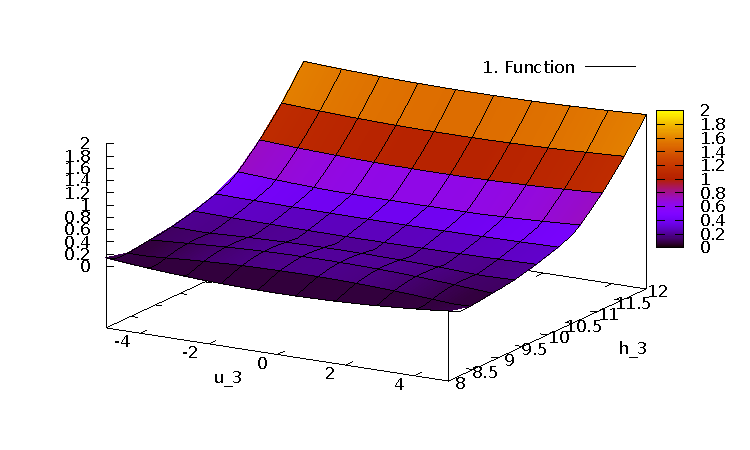
\includegraphics[scale=\zoomfactor]{{{3_punkte_2_hoehe_verringert/0.0_10.0_0.0_10.0_0.0_9.0_0.0_10.0_x_y_0.0_10.0f1}}}  
  }
  \subfigure[Impulse of point $p_1^R$] {
    %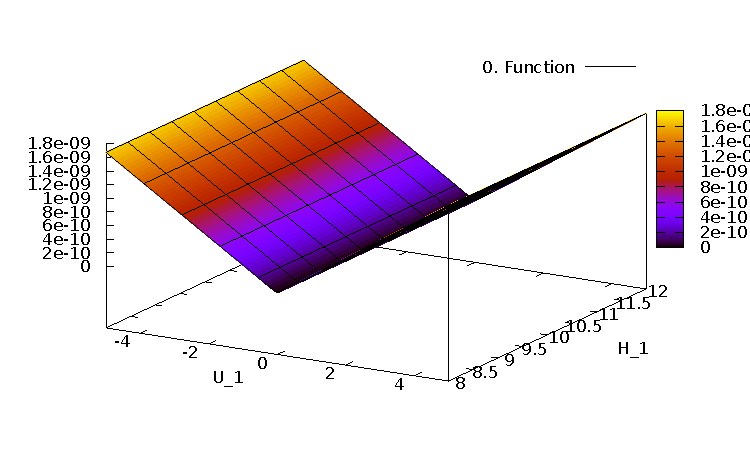
\includegraphics[scale=\zoomfactor]{{{3_punkte_2_hoehe_verringert/0.0_10.0_x_y_0.0_9.0_0.0_10.0_0.0_10.0_0.0_10.0f0}}}  
    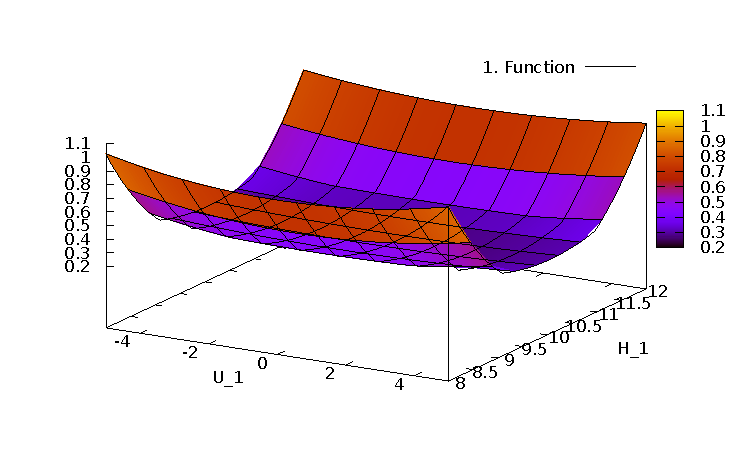
\includegraphics[scale=\zoomfactor]{{{3_punkte_2_hoehe_verringert/0.0_10.0_x_y_0.0_9.0_0.0_10.0_0.0_10.0_0.0_10.0f1}}}  
  }

  \subfigure[Impulse of point $p_2^R$] {
    %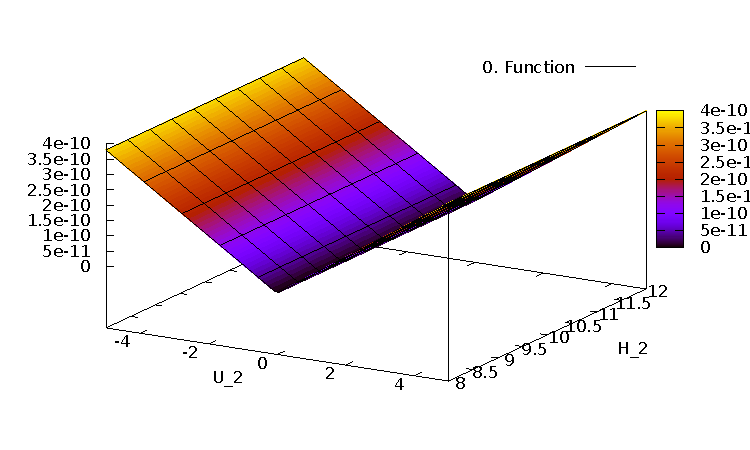
\includegraphics[scale=\zoomfactor]{{{3_punkte_2_hoehe_verringert/0.0_10.0_0.0_10.0_0.0_9.0_x_y_0.0_10.0_0.0_10.0f0}}}  
    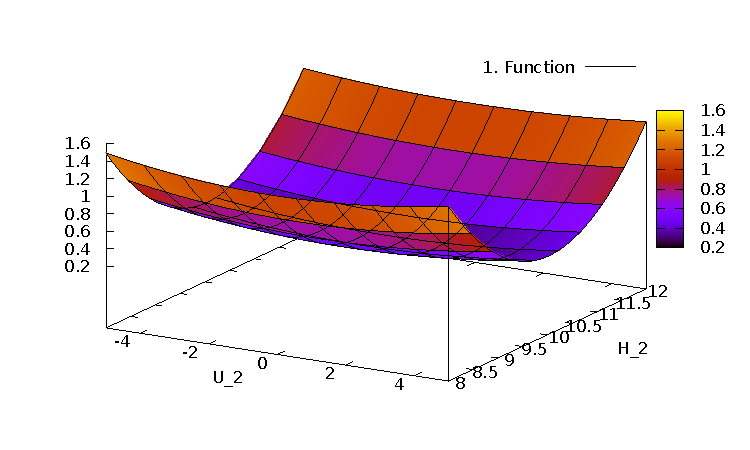
\includegraphics[scale=\zoomfactor]{{{3_punkte_2_hoehe_verringert/0.0_10.0_0.0_10.0_0.0_9.0_x_y_0.0_10.0_0.0_10.0f1}}}  
  }
  \subfigure[Impulse of point $p_3^R$] {
    %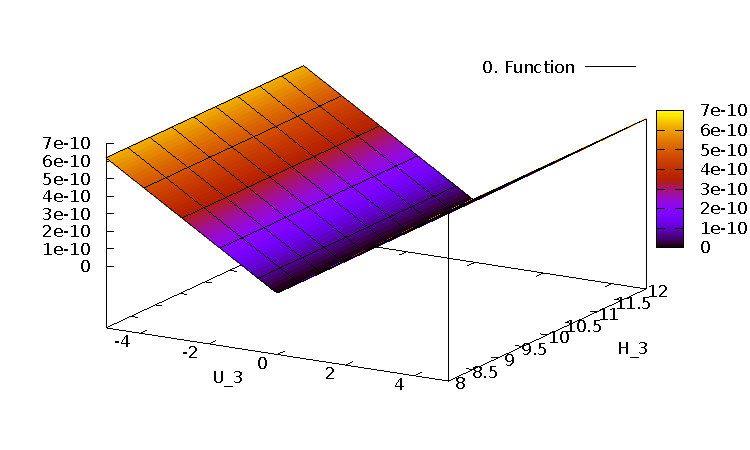
\includegraphics[scale=\zoomfactor]{{{3_punkte_2_hoehe_verringert/0.0_10.0_0.0_10.0_0.0_9.0_0.0_10.0_0.0_10.0_x_yf0}}}  
    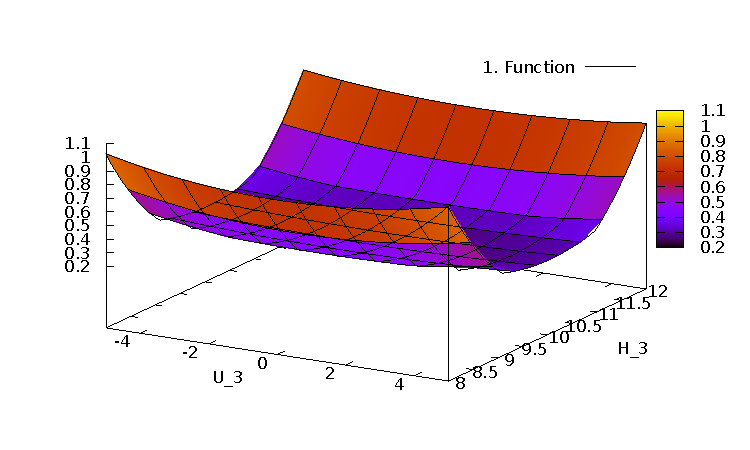
\includegraphics[scale=\zoomfactor]{{{3_punkte_2_hoehe_verringert/0.0_10.0_0.0_10.0_0.0_9.0_0.0_10.0_0.0_10.0_x_yf1}}}  
  }
  \caption{Three points for each triangle. All points except $p_2$ have height 10, impulse 0. Point $p_2$ is set to $(9,0)$. We omit the plots for the $h$-components for other points than $p_1^L$ since the plot has (roughly) the same shape than the one in subfigure \label{subfig:height-p1-three-points-p2-height-decreased} and the error is partially even smaller than $10^{-9}$ for the other points.}
  \label{fig:three-points-h2-}
\end{figure}

%%% Local Variables:
%%% TeX-master: "../results.tex"
%%% End:

%%% Local Variables:
%%% TeX-master: "../results.tex"
%%% End:
